\chapter{相关理论与技术}\label{chap:theories_tech}

% \section{可观测性}

\section{BPF}

eBPF(Extended Berkeley Packet Filter)是Linux内核中的一个轻量级、快速的64位的类RISC虚拟机\citep{sharaf2022extended}。当前eBPF当前已经成为在Linux内核运行时执行不可信的、由用户定义的专用代码的最佳实践与事实标准。其强大的性能、可移植性、灵活性与安全性得到了工业界和学术界的认可,并被广泛地用于更多的领域。

eBPF的前身是BPF(Berkeley Packet Filter),最早由McCanne和Jacobson设计并提出\citep{mccanne1993bsd},起初BPF如其名称所示,用于在Linux网络子系统中对网络包进行灵活处理,而因其本身优异的设计,被Linux内核社区的贡献者扩展到内核的各个子系统中,来对内核功能进行定制化,为了与旧BPF技术进行区分,内核社区将早期的BPF技术成为cBPF(Classic Berkeley Packet Filter),而BPF和eBPF均指代最新的BPF技术,本文在后续说明中也采用这种做法。

BPF本身是一种指令集,最初设计时考虑到安全性与易用性,允许开发者使用C语言的子集进行编写,并能作为一种编译器后端指令集,由GCC等常用编译器编译为字节码\citep{ebpfguidence}。BPF采用字节码的处于两种原因,其一是方便内核验证器对代码进行验证,其二则与Java思想类似,即利用字节码与语言虚拟机的组合提升可移植性。BPF虚拟机运行在内核中,Linux提供了相关的BPF系统调用来将字节码加载到内核中,并附加到代码中声明的钩子函数处,当对应函数触发时,内核态的BPF虚拟机就会执行附加的BPF字节码。整个过程中为了防止加载非法代码,内核首先会在加载BPF代码前对BPF字节码进行验证,判断是否符合在内核中执行的规范,如不允许死循环等,而在内核BPF虚拟机中执行时,会利用JIT技术将字节码映射到本机机器码,从而实现最佳的运行性能。

同作为对内核功能的扩展,BPF技术经常会与内核模块进行比较。相较于内核模块,BPF技术具有更高的安全性,BPF程序安全性体现在三个方面。首先不同于内核模块,BPF程序在编写时所有的对内核数据、地址的访问都需要通过BPF Helper函数来实现,同时,部分BPF Helper函数设计时就考虑到并发性,极大减少了不安全代码的数量。其次,BPF代码在加载时会被内核验证,同时由于运行在虚拟机中,也增强了安全性。最后,BPF代码所能执行的位置由内核提供,这样也大大缩小了危险代码的影响范围。

\begin{figure}[!htbp]
    \centering
    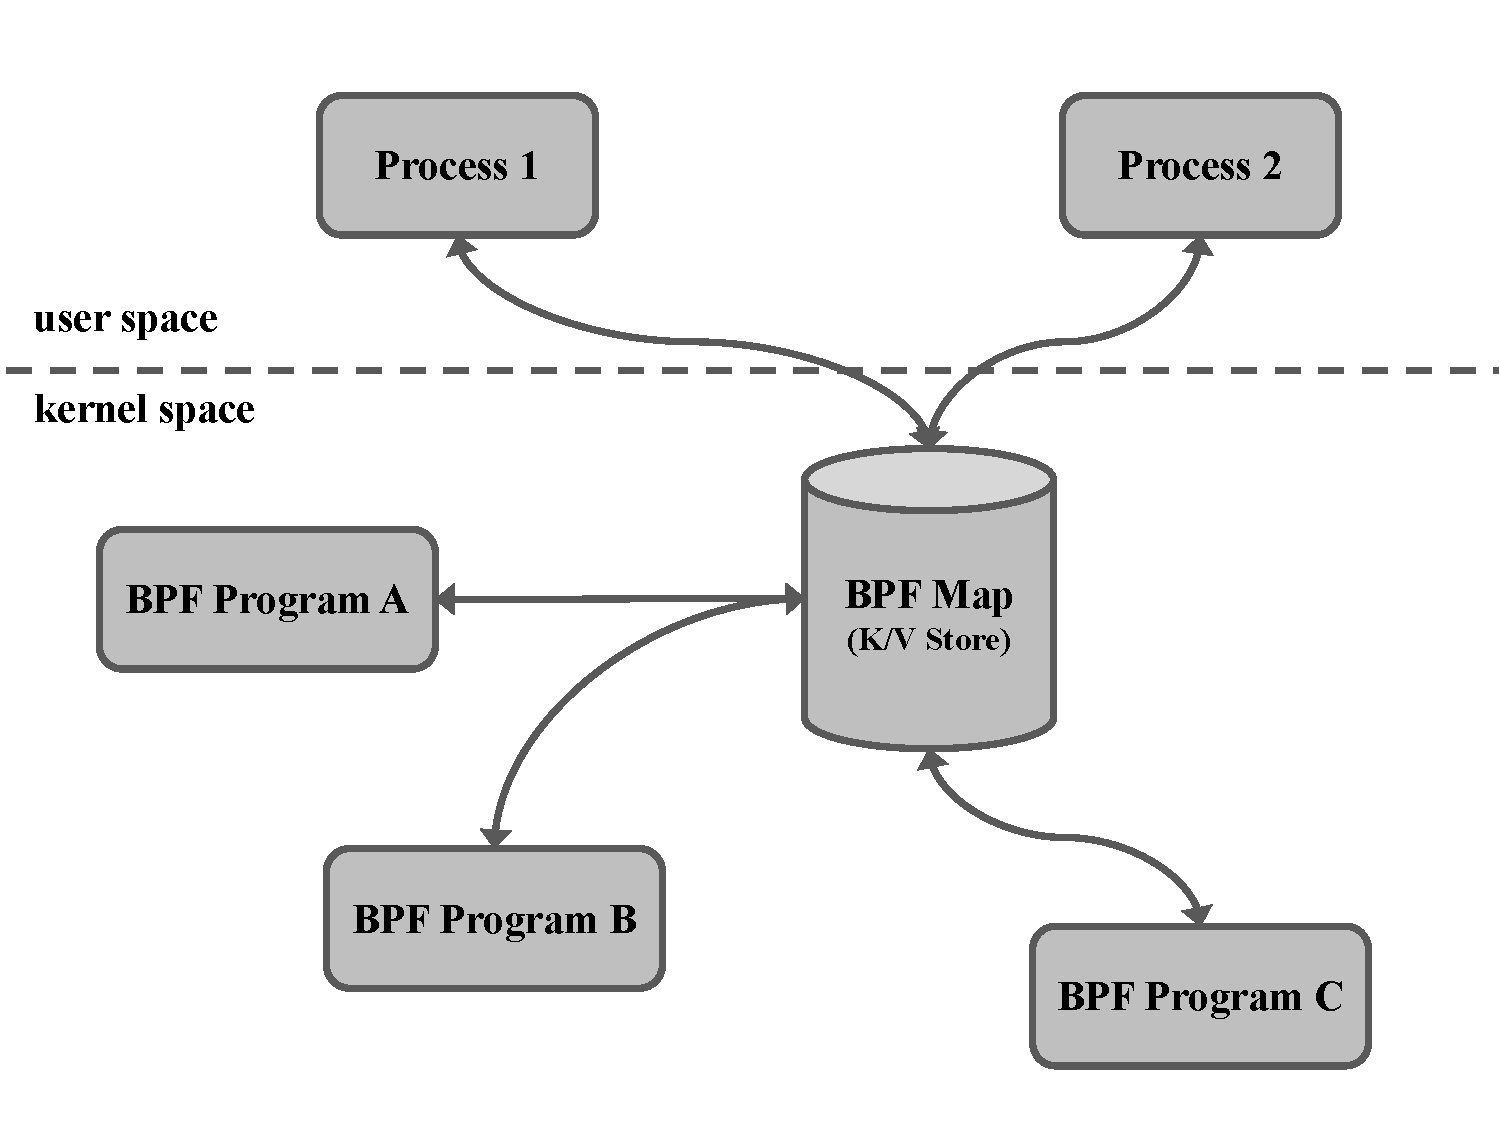
\includegraphics[width=0.8\textwidth]{bpf_user_kernel}
    \bicaption{\quad BPF中用户态与内核态的交互}{\quad Interaction between user mode and kernel mode in BPF}
    \label{fig:bpf_user_kernel}
\end{figure}

同时,BPF技术也具备高度的灵活性。这种灵活性体现在两个方面,首先对于用户态与内核态的交互,BPF技术运行由用户态的程序来加载BPF代码,由于BPF本身是字节码,因此能够借助libbpf等工具来对代码中的部分进行修改,这大大增强了BPF代码的灵活性。其次,BPF技术允许通过BPF Map来实现用户态与内核的逻辑交互,一方面,内核态BPF程序所收集到的数据,能够借助BPF Map反馈给用户态程序进行处理,另一方面用户态程序也能通过BPF系统调用操作内BPF Map,对其中的内容进行读写,从而影响内核态BPF程序的行为。其次,BPF技术还允许BPF程序之间的交互,除上述通过BPF Map的交互外,BPF程序还能够相互进行调用,从而进行数据传递,或通过多个BPF程序的调用,来突破内核对单个BPF函数的限制,从而实现更加复杂的代码逻辑。

\begin{figure}[!htbp]
    \centering
    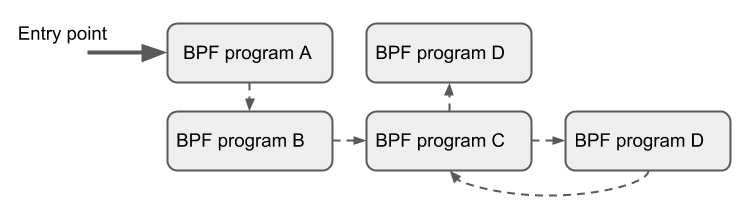
\includegraphics[width=0.8\textwidth]{bpf_to_bpf}
    \bicaption{\quad BPF程序之间的调用}{\quad Interaction between BPF programs}
    \label{fig:bpf_to_bpf}
\end{figure}

然而BPF技术也存在设计上的不足。由于在设计时首要考虑的是安全性,因此BPF程序在编写受到了种种限制,实际上,编写BPF程序所能使用的C语言子集是非图灵完备的,同时BPF程序在栈空间上也有严格的要求。这些限制都极大削弱了BPF程序的表达能力,使得其能够编写的逻辑十分有限。内核社区关注到这一点,并在近期的版本更新中逐步地减少对BPF程序的限制。

\section{Sched Ext}



\section{本章小结}